\chapter{Zustände der VSG-UI in Unity}\label{ch:anhang_ui_workflow}

Die folgenden Abbildungen zeigen die Unity-Benutzungsoberfläche des VSG in ausgewählten Phasen der Generierungspipeline.
Sie veranschaulichen exemplarisch den Initialzustand, den Human-in-the-Loop-Schritt sowie den Consistency-Reviewer-Schritt. Sie ergänzen so die Beschreibung des Ablaufs aus Kapitel~\ref{ch:konzeption_und_implementierung}.

\begingroup
\captionsetup{type=figure,font=small,skip=4pt,list=no}
\begin{center}
	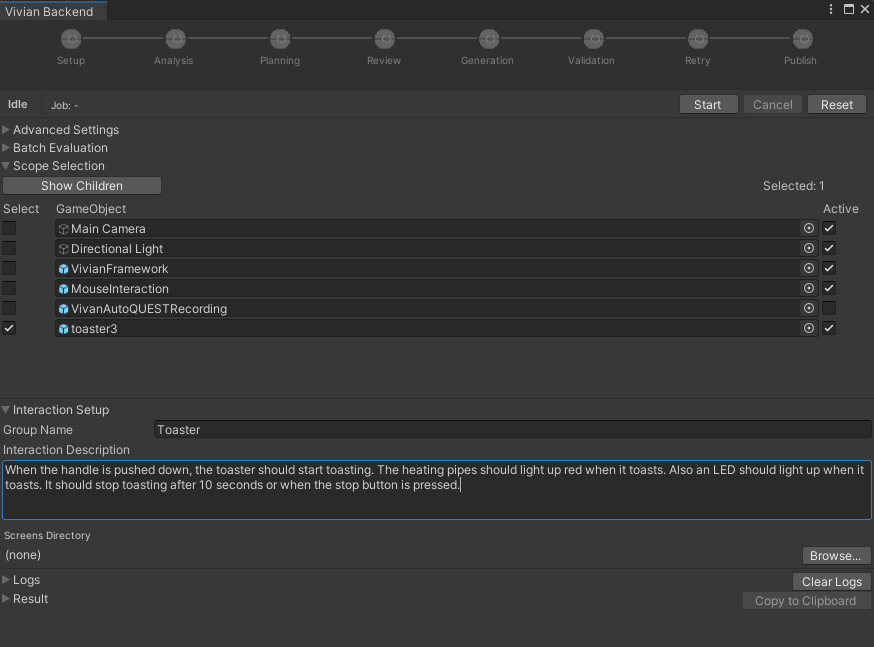
\includegraphics[width=\linewidth]{figures/ui/unity_ui_init}
	\caption{Unity UI des VSG im Initialzustand}\label{fig:ui_init}

	\clearpage

	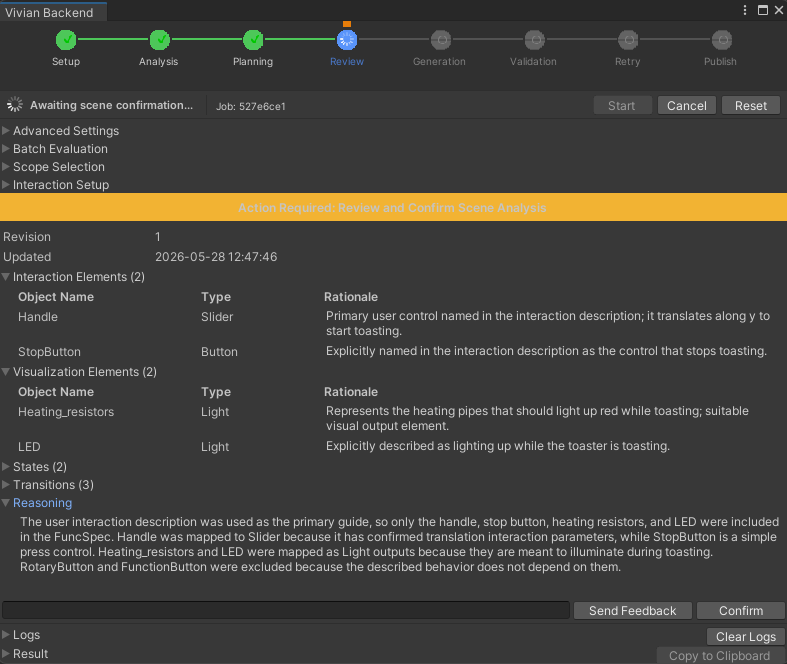
\includegraphics[width=\linewidth]{figures/ui/unity_ui_confirmation_step}
	\caption{Unity UI des VSG im Bestätigungsschritt}\label{fig:ui_confirmation_step}

	\clearpage

	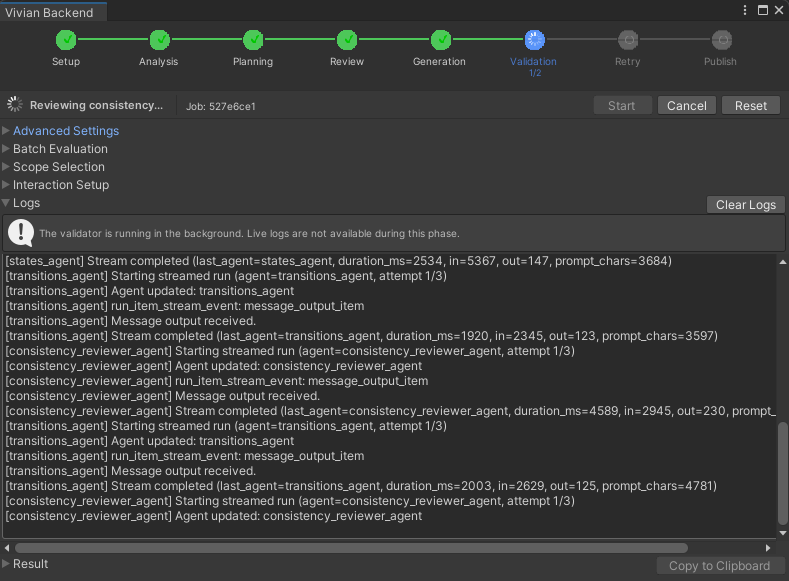
\includegraphics[width=\linewidth]{figures/ui/unity_ui_validation}
	\caption{Unity UI des VSG im Consistency-Reviewer-Schritt}\label{fig:ui_validation}
\end{center}
\endgroup
